\chapauth{leb388}
\chapter{The Girl}



The night was cool and dark, unusual for summer. But then again, it
was a night for unusual things. Slashes of rain whipped at my face
as I navigated the alley. Fireworks vomited sparks of blue and red
into the sky. The booms sounded more like gunshots from Berettas. I
should know; I have one. I am a private detective.



My name is Bavarious. Luke Bavarious.



I'd been at the bar, kicking back a few martinis, when I got a call
about a noise complaint. I work every night if I have to, even the
Fourth of July. The job sounded easy enough, and after all, the
people need me. I am their protector. I am Luke Bavarious.



But on this night, I wasn't as alone as I thought. As I walked
along, I heard the sound of footsteps. I stopped. ``Who's there?'' I
yelled, raising my Beretta.



No response.



I tensed. ``Come out where I can see you,'' I ordered. ``Now.''



A child stepped out of the shadows and into the trashy street. I
say that because the street was littered with trash. The people
there were usually nice.



Most of the time.



I holstered the Beretta, at ease. The girl looked young. Maybe six,
could even be seven. Who knows, in this town. Probably lost. She
clutched a doll and wore a dark raincoat. Not like that was any
help, in this torrential weather.



``Are you okay?'' I asked her. ``Do you need help?''



``I need to find my mommy,'' she whimpered. She was crying.



A girl that young shouldn't be alone in an alley off 42nd St. in
New York. Especially on a night like tonight. I pulled out my phone
to call to see if anyone reported her missing, but something was
wrong. I looked up at the sky. Fireworks still going at it like
crazy missiles exploding in the air. That's what they were.
Missiles. And that's when I saw it. The creature. The item the girl
was holding wasn't a doll after all--it was a monster. It had
buttons for eyes. There was no mouth, just stitches. The hair was
yarn.



``Get out of here, fiend of hell!'' I screamed.



I grabbed it. If you can call it an it. The hands were soft. At
least until I flung it into the puddle. Then they were wet. I
screamed, shooting at it with my Beretta. I felt a fear no one
should ever have to experience, a fear of the worst possible
things, a fear of death and everything around it. It was taking
hold of me, drowning me, and I kept spinning and spinning in the
abyss of its grip. I felt like vomiting. Maybe that was just from
the martinis. I shot it again and again, and so on. And then I
stopped.



A flash of light made me see its face. Kind. Adorable. Just a doll
after all.



Why do I always investigate noise complaints when I'm drunk?
Suddenly, the girl was sobbing. And I felt like an asshole. 

 


\begin{figure}[b]
  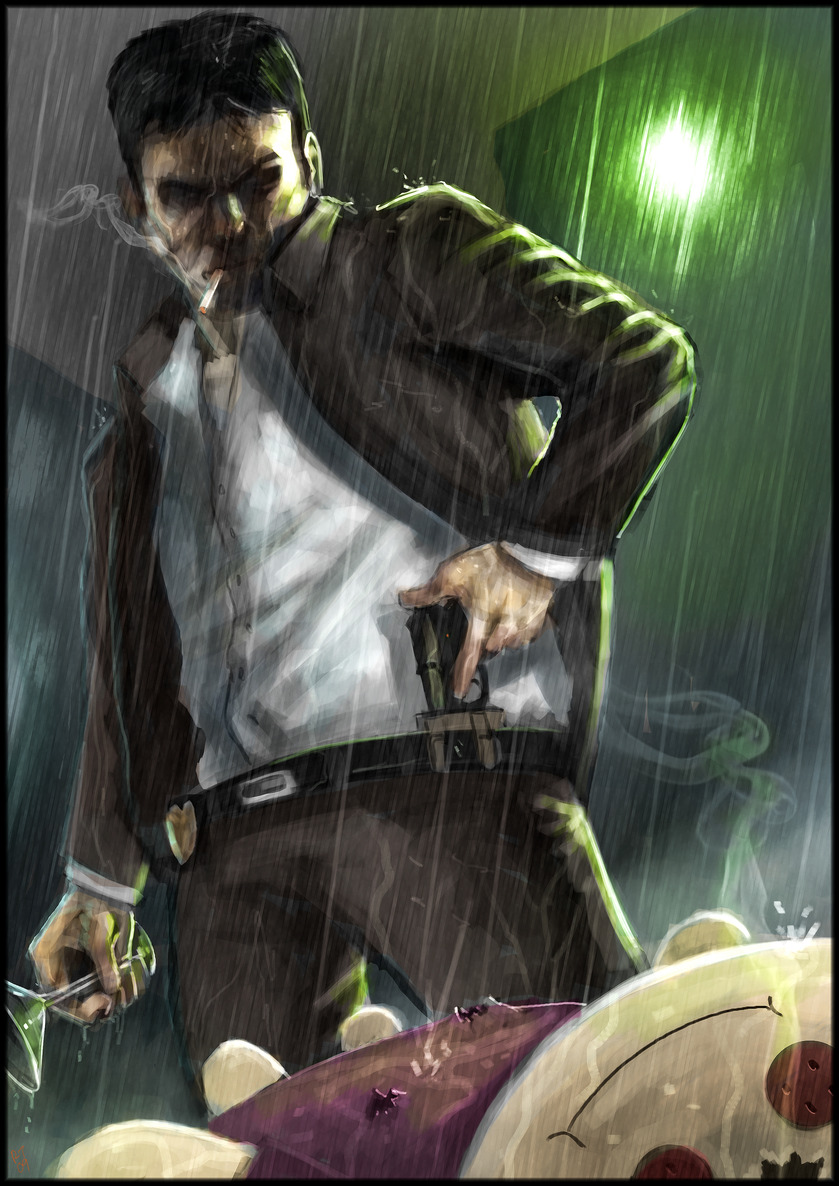
\includegraphics[width=\textwidth]{art/Discount_Bees-The_Girl.jpg}
  \caption{{\em The Girl} by Discount\_Bees}
\end{figure}
